\chapter{Results \label{ch:results}}
The ID lines are analysed by the program \verb|att_eval.py| introduced in section \ref{sec:meth:data_interpretation}. The

\section{Calibration \label{sec:res:calibration}}
The unfiltered measurements of the magnetometer are presented in fig. \ref{fig:res:raw_cali}. Three bigger spots can be seen, which do not lay on the sphere, as well as some single measurement points distributed throughout the figure. The first step is to eliminate these statistical outliers.

\begin{figure}[H]
    \centering
    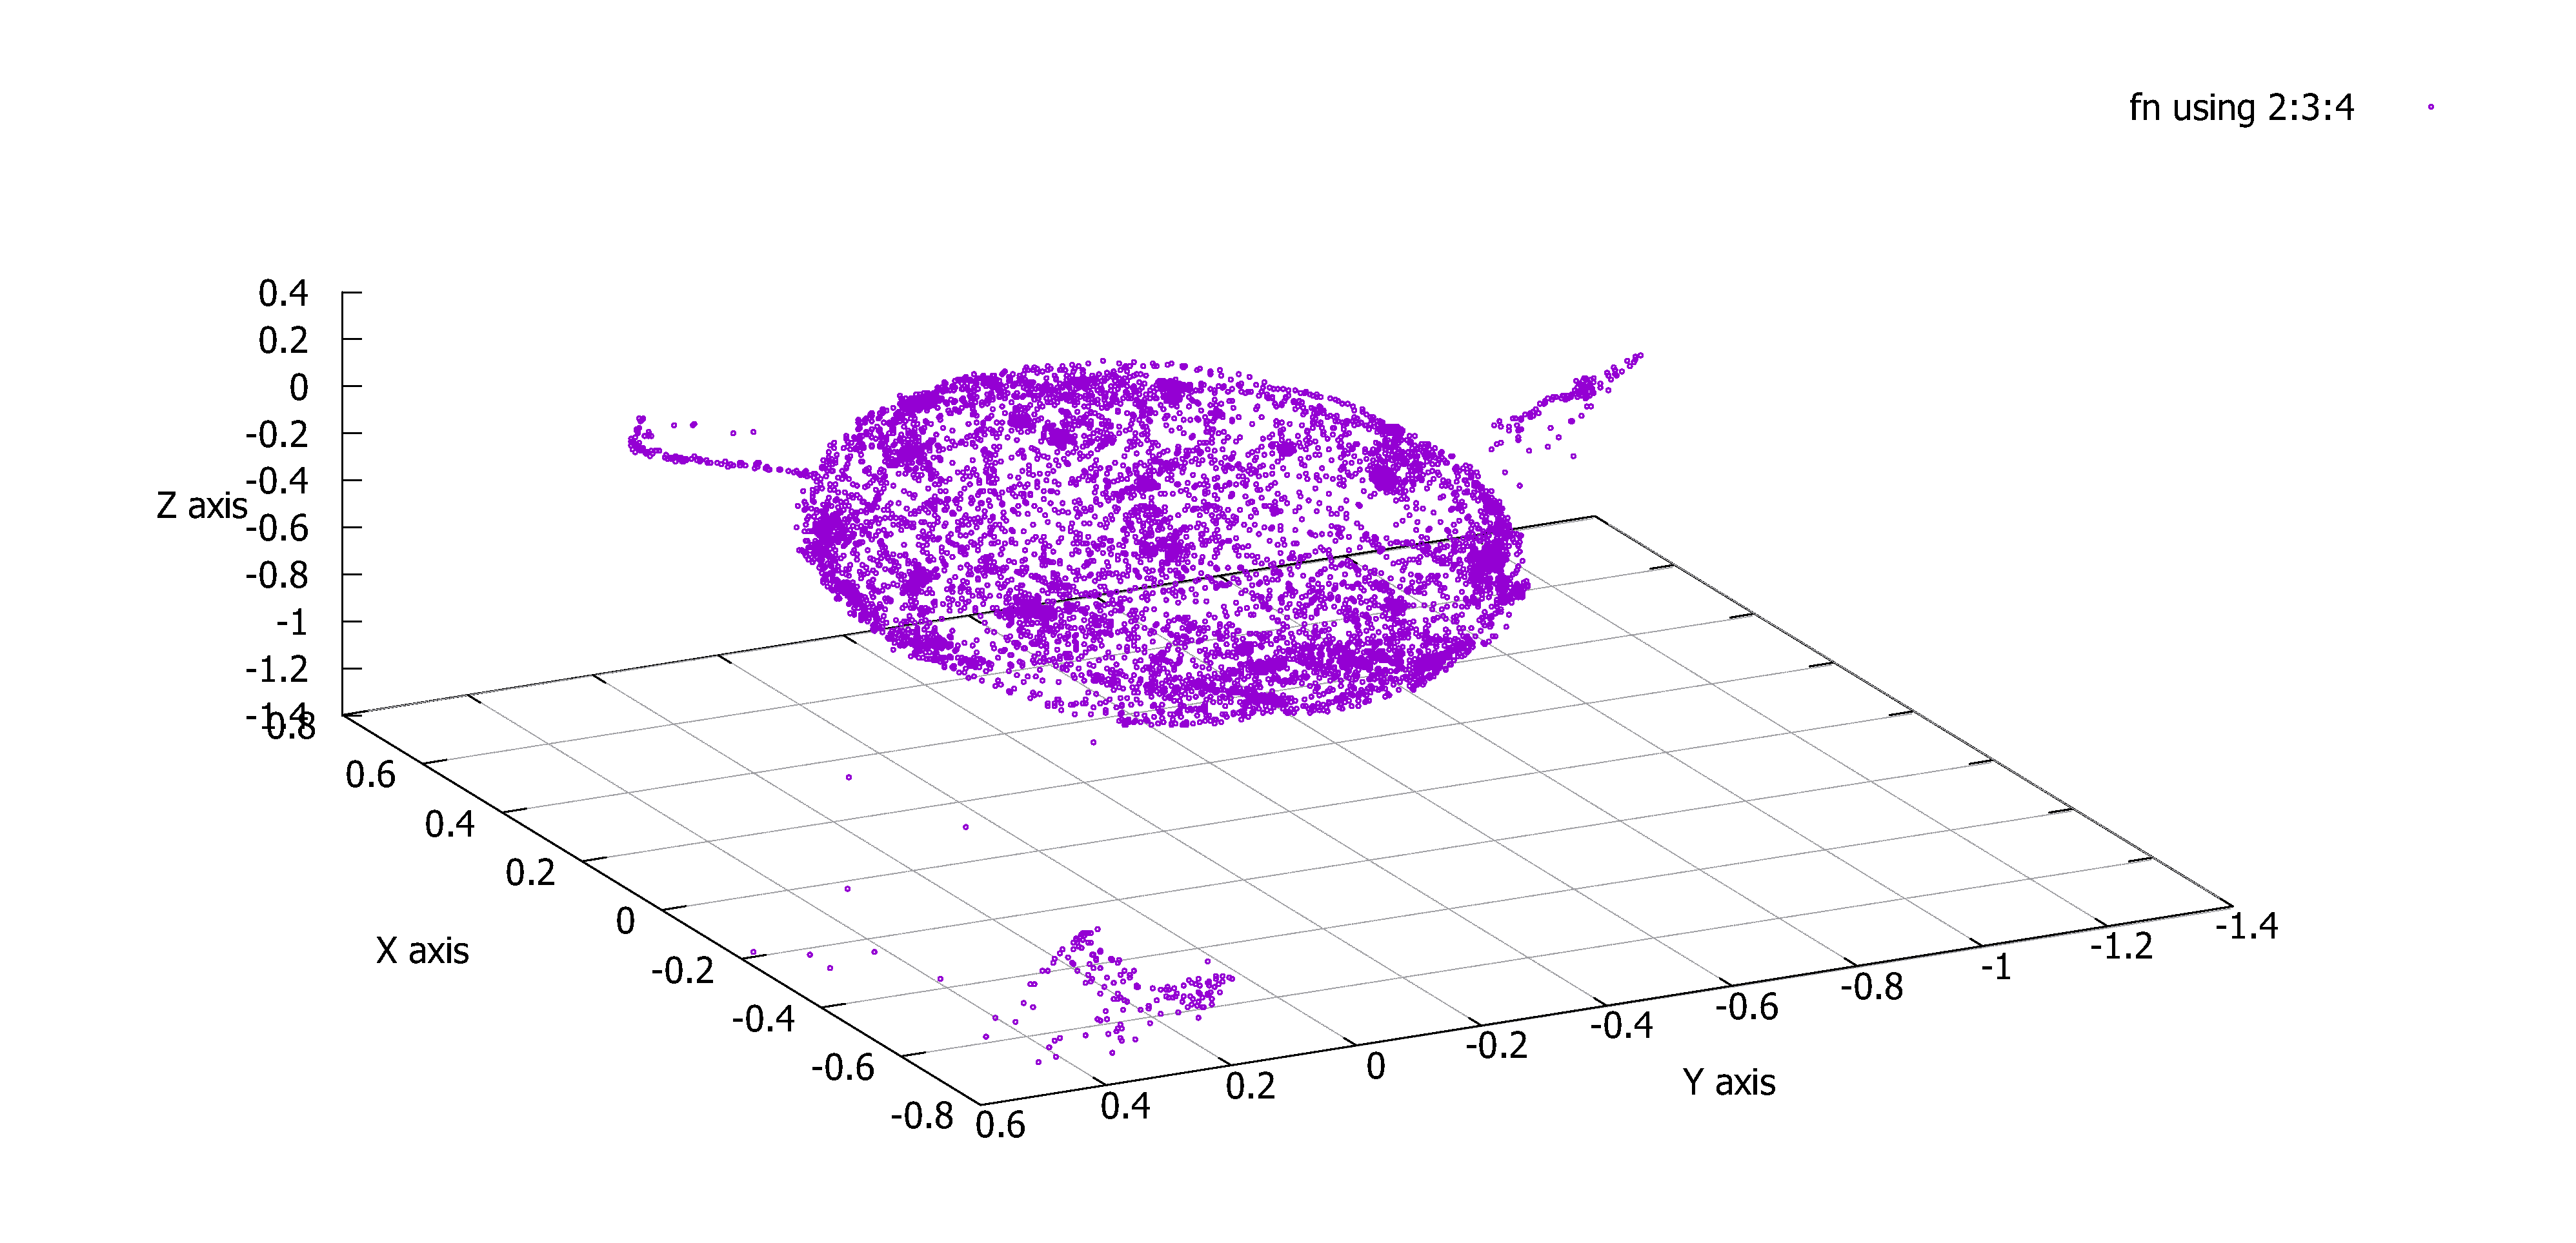
\includegraphics[width=0.8\linewidth]{images/04_results/raw_sphere_2025-04-11.pdf}
    \caption{Components of the magnetometer of the calibration measurement on 11 April 2025 plotted in 3D-Space to form a distorted sphere.}
    \label{fig:res:raw_cali}
\end{figure}

In fig. \ref{fig:res:raw_cali_vectors} the three components of the magnetometer and accelerometer are plotted against their timestamp. This time is incorrect, as the \ac{FPGA} simply continues counting up from the last time it was connected to the internet. That the timestamp is incorrect does not matter for the sensor calibration, as only the time order of the vectors is relevant. In the figure there can be made a clear distinction between three time intervals. The first interval is from the beginning of the measurement until 9:55. This is the time it took to leave the lab, take the elevator to the basement and go to the car park. A lot of vibration can be seen in the accelerometer and stray magnetic fields measured by the magnetometer.\\
The second phase is from 9:55 to around 10:21, when the random tumble begins. In this phase it can be seen how the magnetometer and accelerometer react to laying the device housing down in different orientations. When rotating the sensors, small shocks can be seen, such as at 10:05 when the magnetometer is turned so that the earth's magnetic field aligns with the x-axis.

\begin{figure}[H]
    \centering
    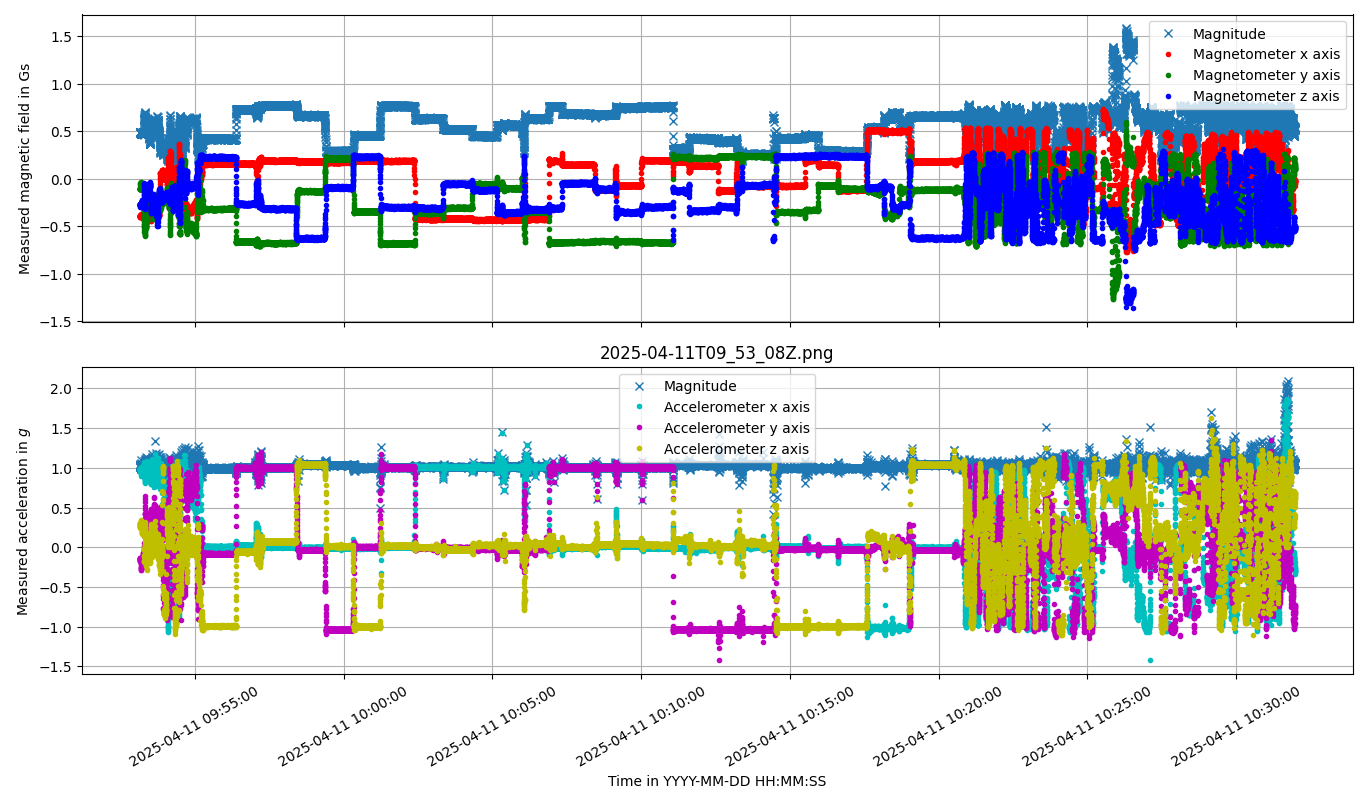
\includegraphics[width=\linewidth]{images/04_results/raw_vectors-2025-04-11.png}
    \caption[Components of the magnetometer and accelerometer plotted against time.]{Components of the magnetometer and accelerometer plotted against time. Shown with blue crosses is the sum of the squares of the components, i.e. the length of the measured vector.}
    \label{fig:res:raw_cali_vectors}
\end{figure}

There is one very important thing we can learn from figure \ref{fig:res:raw_cali_vectors}. The magnetometer measurements are shockingly unreliable. Firstly it can be seen that no particularly sudden or strong accelerations are experienced during the random tumble. However for some reason the magnetometers measured field goes up to about 1.5\,Gs which is around 6 times the field in Kiel (see sec. \ref{sec:da:vector_fields}). Secondly the measured field's magnitude should be roughly constant throughout the whole time of phases two and three when the device is brought outside, away from any hard iron sources. However looking at 10:00 it is blatantly obvious that this is not the case at all.\\
We will perform three approximations of the calibration parameters. The first only taking phase 2 into account, the second only taking phase three into account and the third approximation with both phases. In fig. \ref{fig:res:raw_calibration_three_phases} the components of the magnetometer are shown in all three dimensions to illustrate the different measurement methods of placing the magnetometer in a single position for a longer duration of time (fig. \ref{fig:res:raw_calibration_three_phase_II}) and the random tumble (fig. \ref{fig:res:raw_calibration_three_phase_III}).

\begin{figure}[h]
\begin{subfigure}[t]{.33\textwidth}
  \centering
  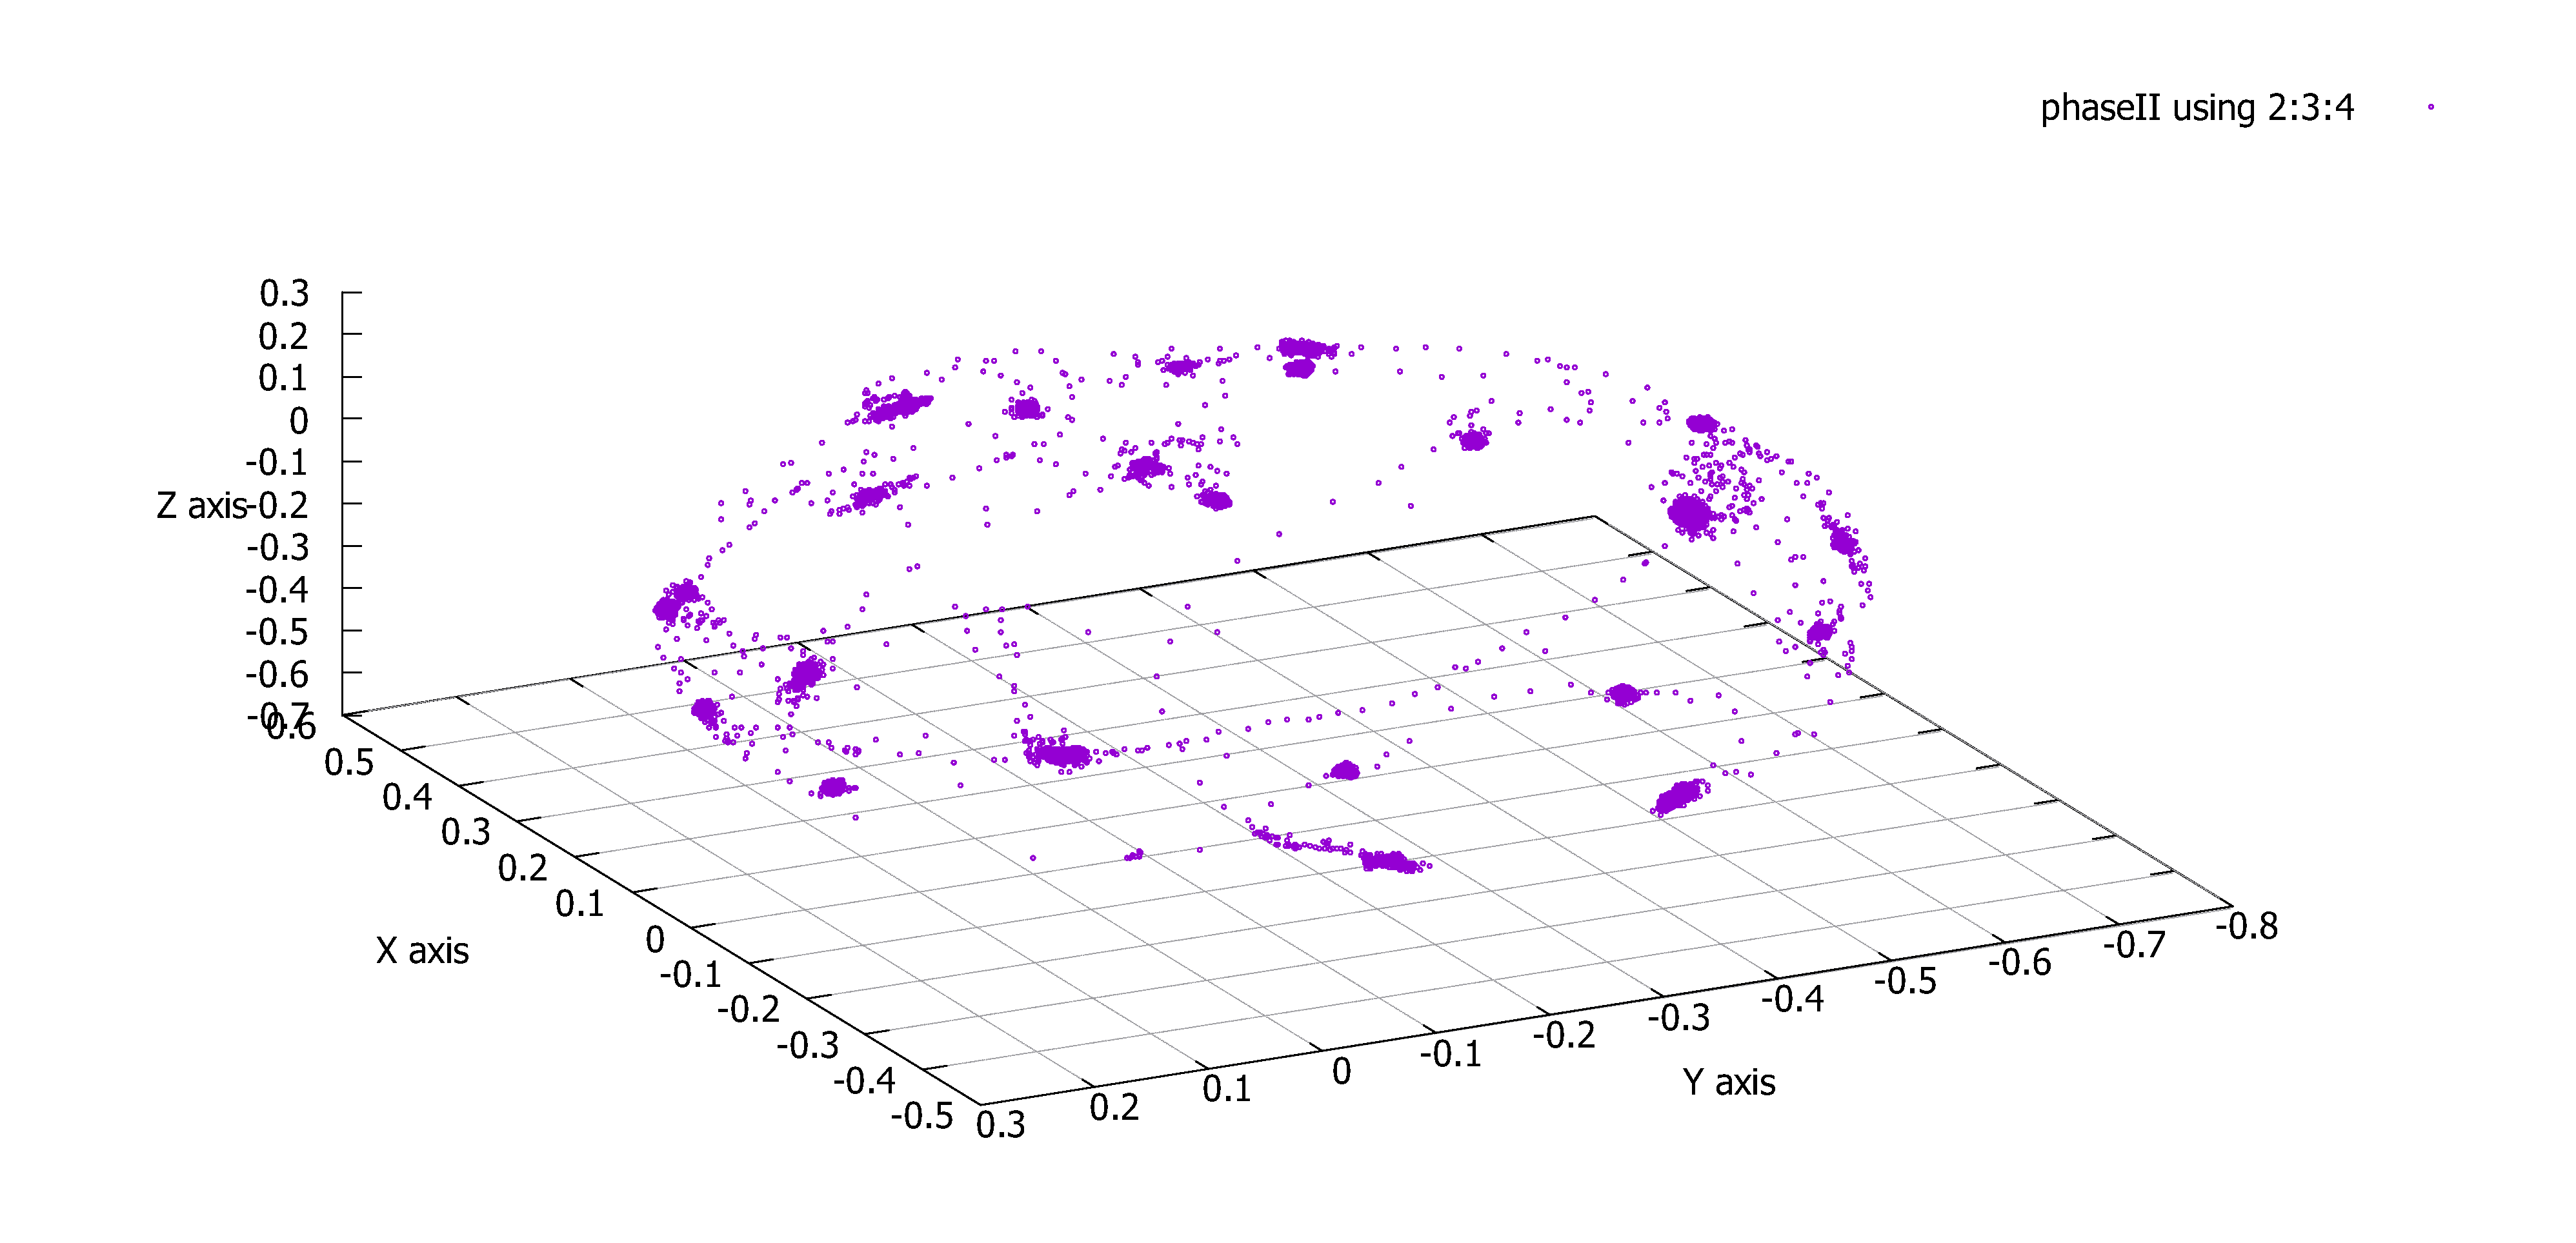
\includegraphics[width=.8\linewidth]{images/04_results/raw_sphere_calibration_phase_II.pdf}
  \caption{Phase II, multiple orientations.}
  \label{fig:res:raw_calibration_three_phase_II}
\end{subfigure}%
\begin{subfigure}[t]{.33\textwidth}
  \centering
  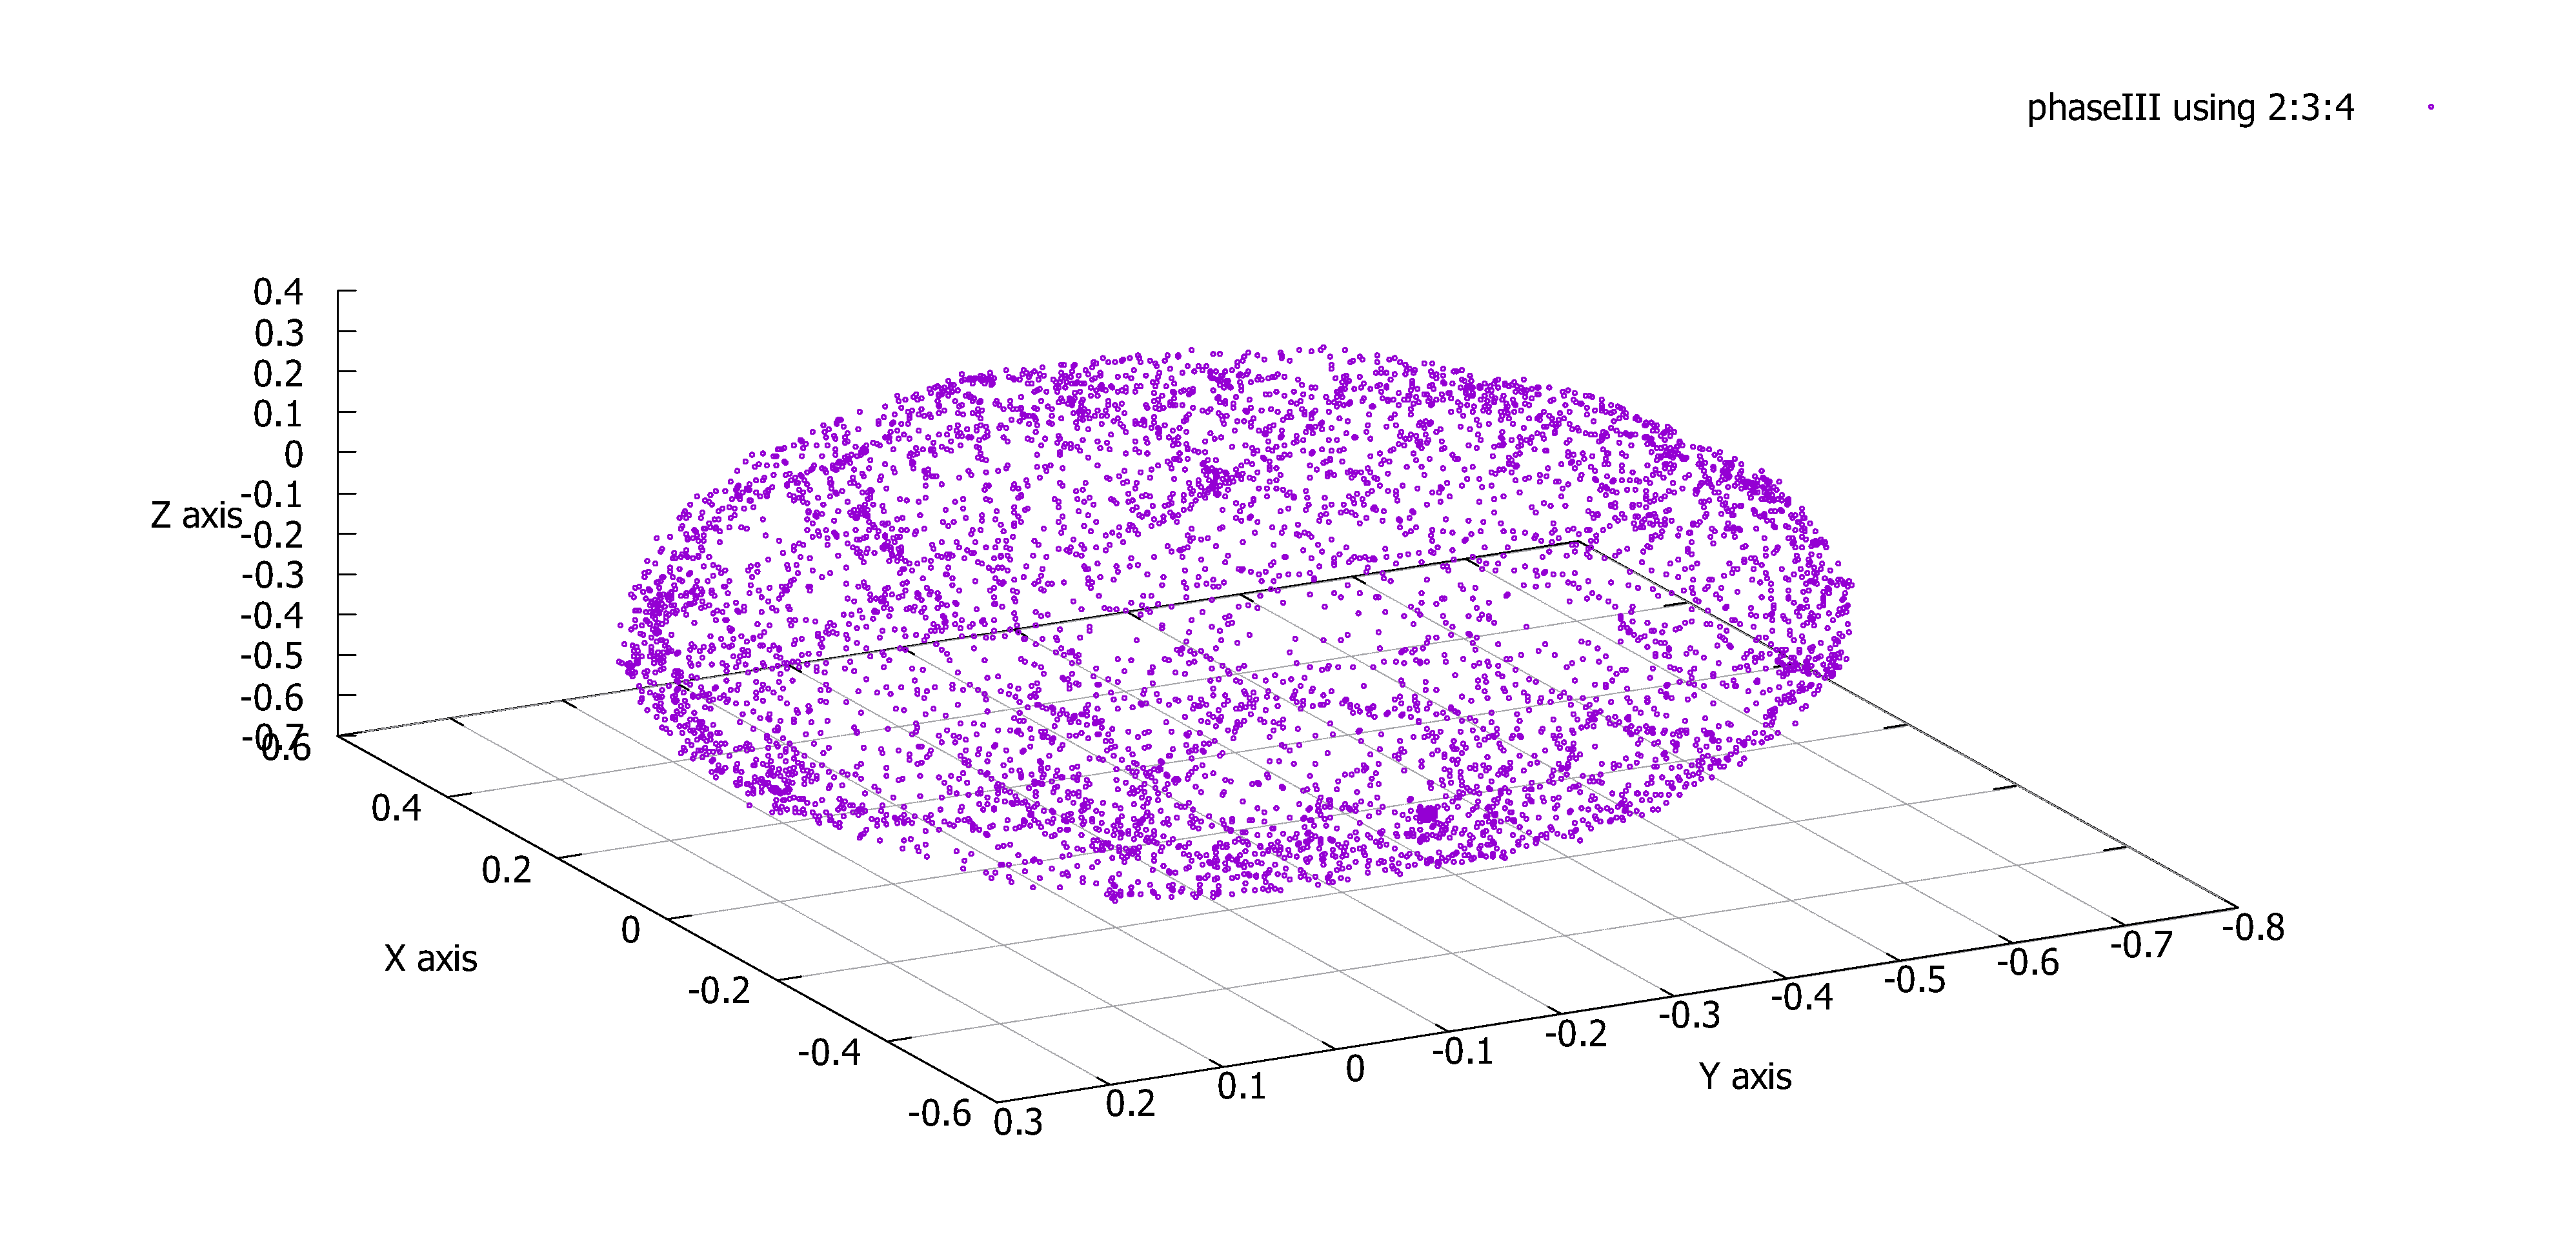
\includegraphics[width=.8\linewidth]{images/04_results/raw_sphere_calibration_phase_III.pdf}
  \caption{Phase III, random tumble.}
  \label{fig:res:raw_calibration_three_phase_III}
\end{subfigure}
\begin{subfigure}[t]{.33\textwidth}
  \centering
  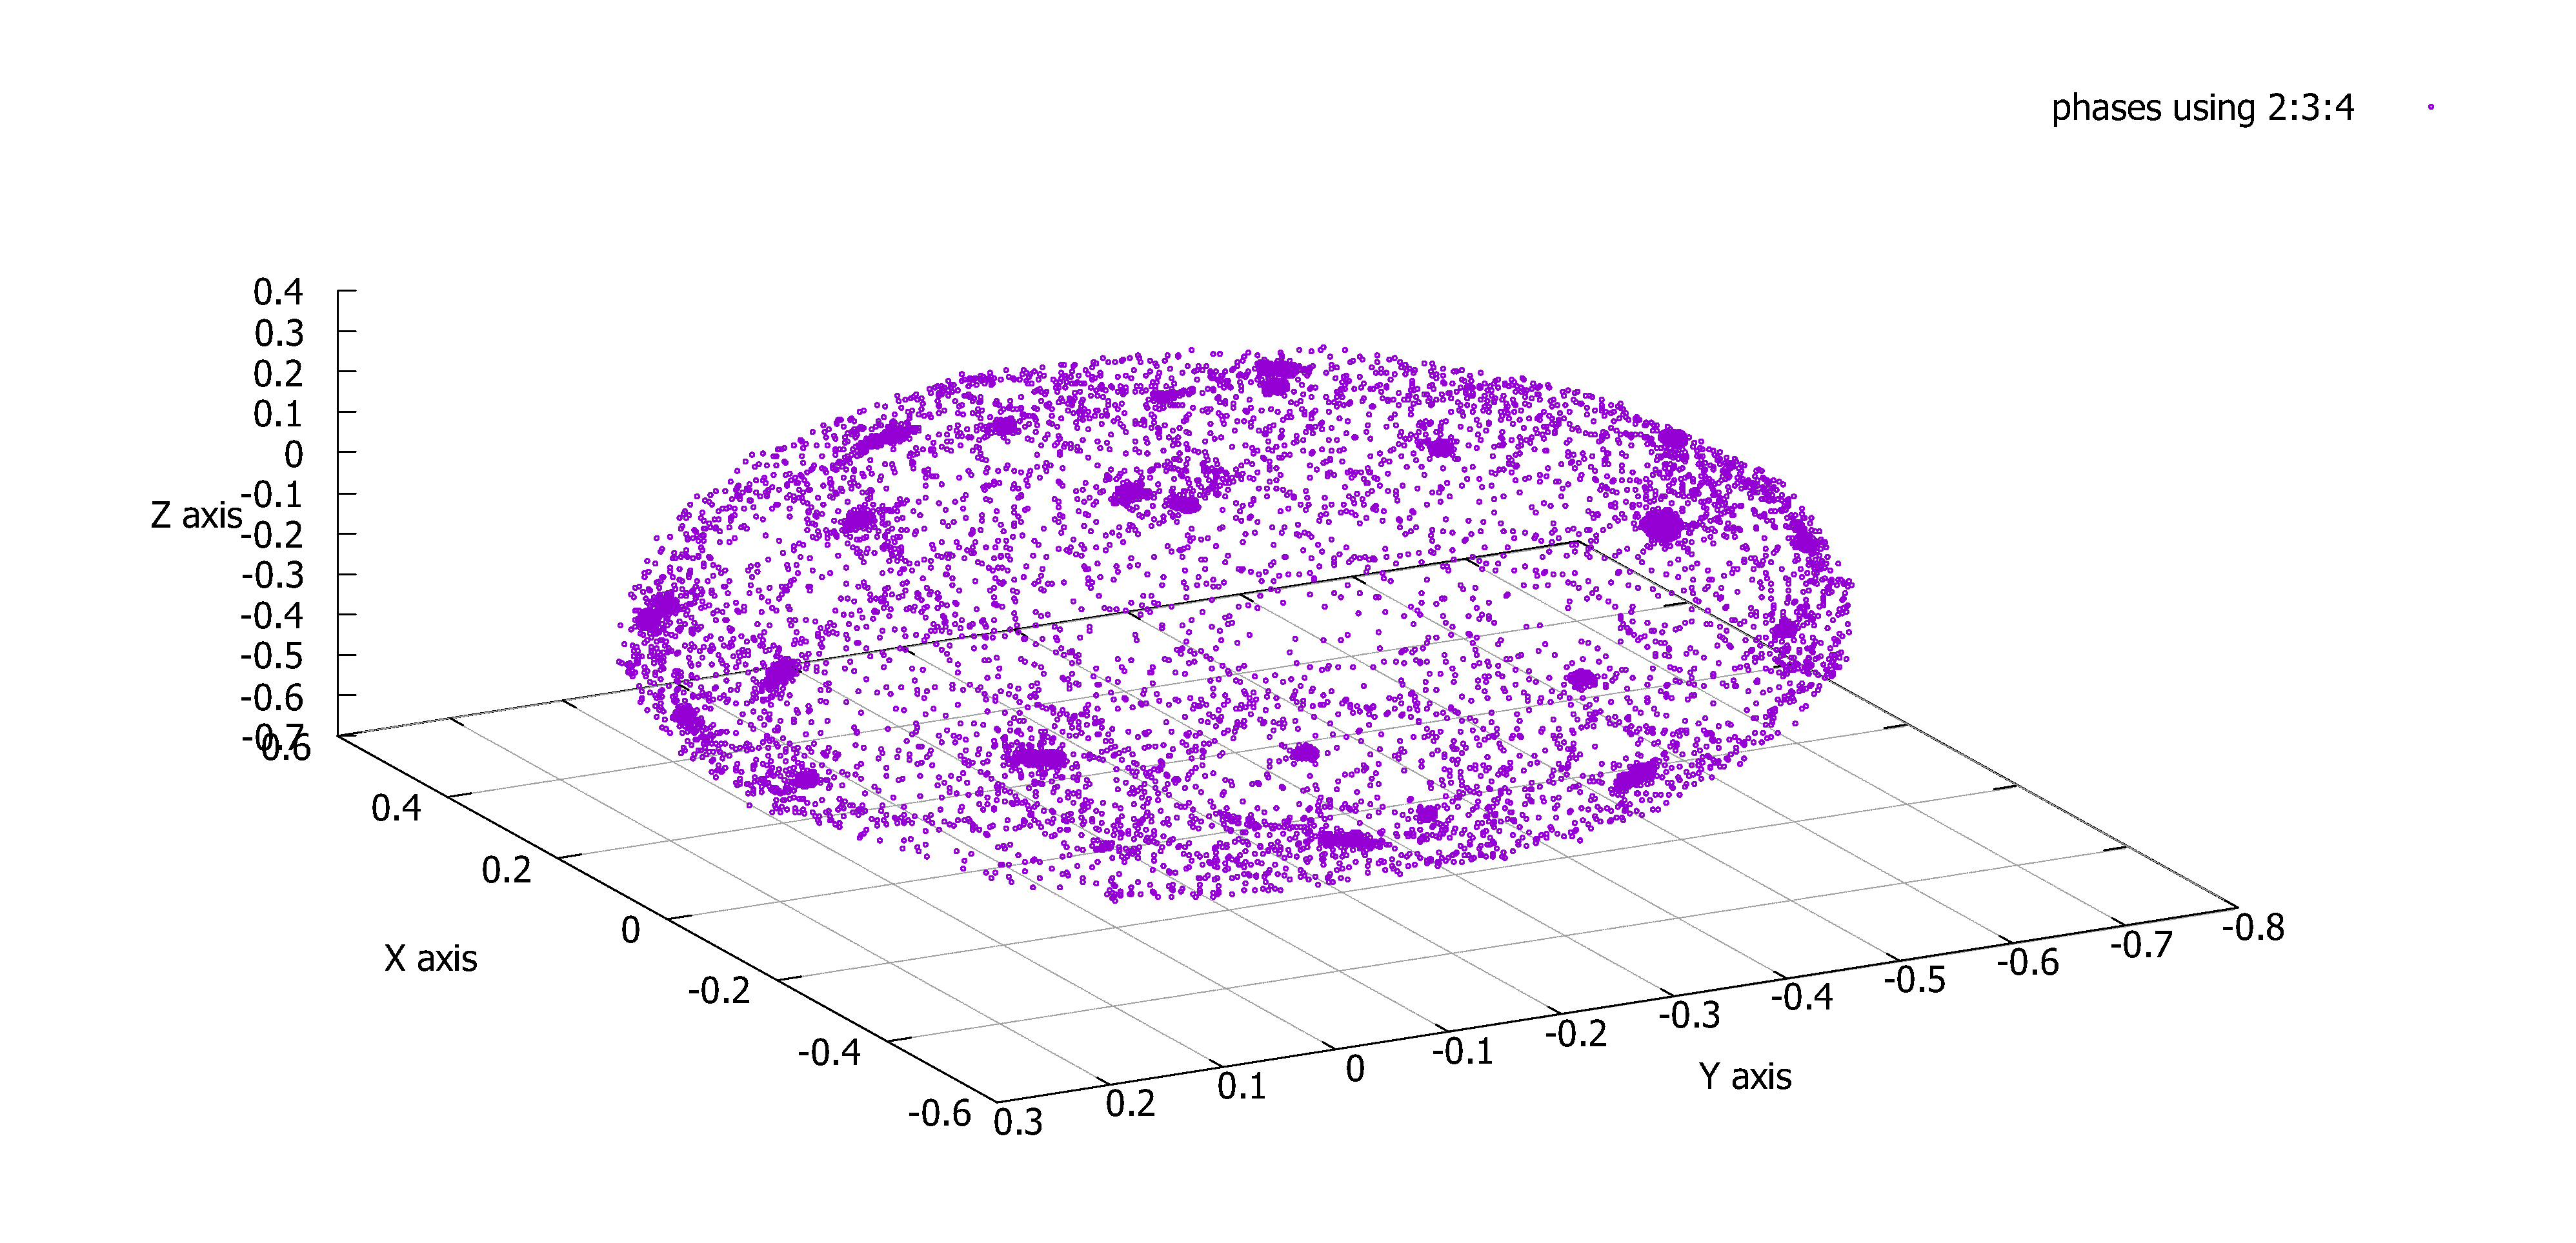
\includegraphics[width=.8\linewidth]{images/04_results/raw_sphere_calibration_phases_II_III.pdf}
  \caption{Phases II and III, combination of both.}
\end{subfigure}
\caption{Magnetometer components of the calibration measurement plotted in 3D-Space to form a distorted sphere.}
\label{fig:res:raw_calibration_three_phases}
\end{figure}


The final coefficients are:
\begin{table}
    \centering
    \begin{tabular}{c|c|c|c}
         \thead{Coefficient} & \thead{Phase II} & \thead{Phase III} & \thead{Phases II + III} \\ \hline
         \makecell{$a^B$} & \makecell{1.02394} & \makecell{1.00341} & \makecell{1.03179} \\
         \makecell{$b^B$} & \makecell{1.08484} & \makecell{1.06898} & \makecell{1.07573} \\
         \makecell{$c^B$} & \makecell{1.18253} & \makecell{1.12627} & \makecell{1.16176} \\
         \makecell{$x_0^B$} & \makecell{0.0344209} & \makecell{0.0131758} & \makecell{0.0269842} \\
         \makecell{$y_0^B$} & \makecell{-0.22116} & \makecell{-0.212521} & \makecell{-0.219484} \\
         \makecell{$z_0^B$} & \makecell{-0.195463} & \makecell{-0.192554} & \makecell{-0.195859} \\
         \hline
         \makecell{$a^g$} & \makecell{0.969417} & \makecell{0.978286} & \makecell{0.97323} \\
         \makecell{$b^g$} & \makecell{0.959791} & \makecell{0.948732} & \makecell{0.957992} \\
         \makecell{$c^g$} & \makecell{0.964618} & \makecell{0.926156} & \makecell{0.953446} \\
         \makecell{$x_0^g$} & \makecell{-0.00218403} & \makecell{0.00733717} & \makecell{0.00149607} \\
         \makecell{$y_0^g$} & \makecell{-0.0149083} & \makecell{-0.0113024} & \makecell{-0.014287} \\
         \makecell{$z_0^g$} & \makecell{0.0218019} & \makecell{0.0260466} & \makecell{0.0251443} \\
    \end{tabular}
    \caption{Coefficents determined from measurement on 11 April 2025.}
    \label{tab:res:coeff}
\end{table}

\begin{table}
    \centering
    \begin{tabular}{c|c|c|c|c|c|c}
             &   xa0  &   ya0  &   za0  &   aa   &   ba   & ca \\
         xa0 &  1     &        &        &        &        &    \\
         ya0 & -0.005 &  1     &        &        &        &    \\
         za0 &  0.016 &  0.007 &  1     &        &        &    \\
         aa  &  0.522 & -0.000 &  0.005 &  1     &        &    \\
         ba  &  0.010 &  0.251 &  0.011 &  0.003 &  1     &    \\
         ca  & -0.008 & -0.015 & -0.273 & -0.007 & -0.013 &  1 \\
    \end{tabular}
    \caption{Correlation matrix of Phase II Acc}
    \label{tab:my_label}
\end{table}

\begin{table}
    \centering
    \begin{tabular}{c|c|c|c|c|c|c}
             &   xm0  & ym0    &   zm0  &   am   &   bm   & cm \\
         xm0 &  1     &        &        &        &        &    \\
         ym0 &  0.096 &  1     &        &        &        &    \\
         zm0 &  0.114 &  0.013 &  1     &        &        &    \\
         am  & -0.457 & -0.055 & -0.105 &  1     &        &    \\
         bm  &  0.180 & -0.212 & -0.045 & -0.212 &  1     &    \\
         cm  &  0.229 &  0.065 &  0.282 & -0.252 & -0.093 & 1  \\
    \end{tabular}
    \caption{Correlation matrix of Phase II Mag}
    \label{tab:my_label}
\end{table}

\begin{table}
    \centering
    \begin{tabular}{c|c|c|c|c|c|c}
             &   xa0  &   ya0  &   za0  &   aa   &   ba   & ca \\
         xa0 &  1     &        &        &        &        &    \\
         ya0 &  0.030 &  1     &        &        &        &    \\
         za0 &  0.093 &  0.017 &  1     &        &        &    \\
         aa  & -0.246 & -0.004 &  0.047 &  1     &        &    \\
         ba  & -0.021 & -0.034 & -0.055 & -0.229 &  1     &    \\
         ca  & -0.017 &  0.053 &  0.280 & -0.098 & -0.195 &  1 \\
    \end{tabular}
    \caption{Correlation matrix of Phase III Acc}
    \label{tab:my_label}
\end{table}

\begin{table}
    \centering
    \begin{tabular}{c|c|c|c|c|c|c}
             &   xm0  & ym0    &   zm0  &   am   &   bm   & cm \\
         xm0 &  1     &        &        &        &        &    \\
         ym0 &  0.053 &  1     &        &        &        &    \\
         zm0 &  0.006 &  0.009 &  1     &        &        &    \\
         am  &  0.266 &  0.015 & -0.033 &  1     &        &    \\
         bm  & -0.013 & -0.073 &  0.014 & -0.234 &  1     &    \\
         cm  & -0.017 & -0.046 & -0.222 & -0.185 & -0.203 & 1  \\
    \end{tabular}
    \caption{Correlation matrix of Phase III Mag}
    \label{tab:my_label}
\end{table}

\begin{table}
    \centering
    \begin{tabular}{c|c|c|c|c|c|c}
             &   xa0  &   ya0  &   za0  &   aa   &   ba   & ca \\
         xa0 &  1     &        &        &        &        &    \\
         ya0 & -0.001 &  1     &        &        &        &    \\
         za0 &  0.067 &  0.004 &  1     &        &        &    \\
         aa  &  0.283 & -0.008 &  0.049 &  1     &        &    \\
         ba  & -0.029 &  0.206 &  0.012 & -0.058 &  1     &    \\
         ca  & -0.053 & -0.008 & -0.127 & -0.065 & -0.046 &  1 \\
    \end{tabular}
    \caption{Correlation matrix of Phases II+III Acc}
    \label{tab:my_label}
\end{table}

\begin{table}
    \centering
    \begin{tabular}{c|c|c|c|c|c|c}
             &   xm0  & ym0    &   zm0  &   am   &   bm   & cm \\
         xm0 &  1     &        &        &        &        &    \\
         ym0 &  0.074 &  1     &        &        &        &    \\
         zm0 &  0.057 &  0.002 &  1     &        &        &    \\
         am  & -0.229 & -0.022 & -0.070 &  1     &        &    \\
         bm  &  0.135 & -0.190 & -0.039 & -0.199 &  1     &    \\
         cm  &  0.142 &  0.038 &  0.134 & -0.215 & -0.121 & 1  \\
    \end{tabular}
    \caption{Correlation matrix of Phases II+III Mag}
    \label{tab:my_label}
\end{table}

%%% HOW TO SUBFIGURE %%%
%\begin{figure}[h]
%\begin{subfigure}{.33\textwidth}
%  \centering
%  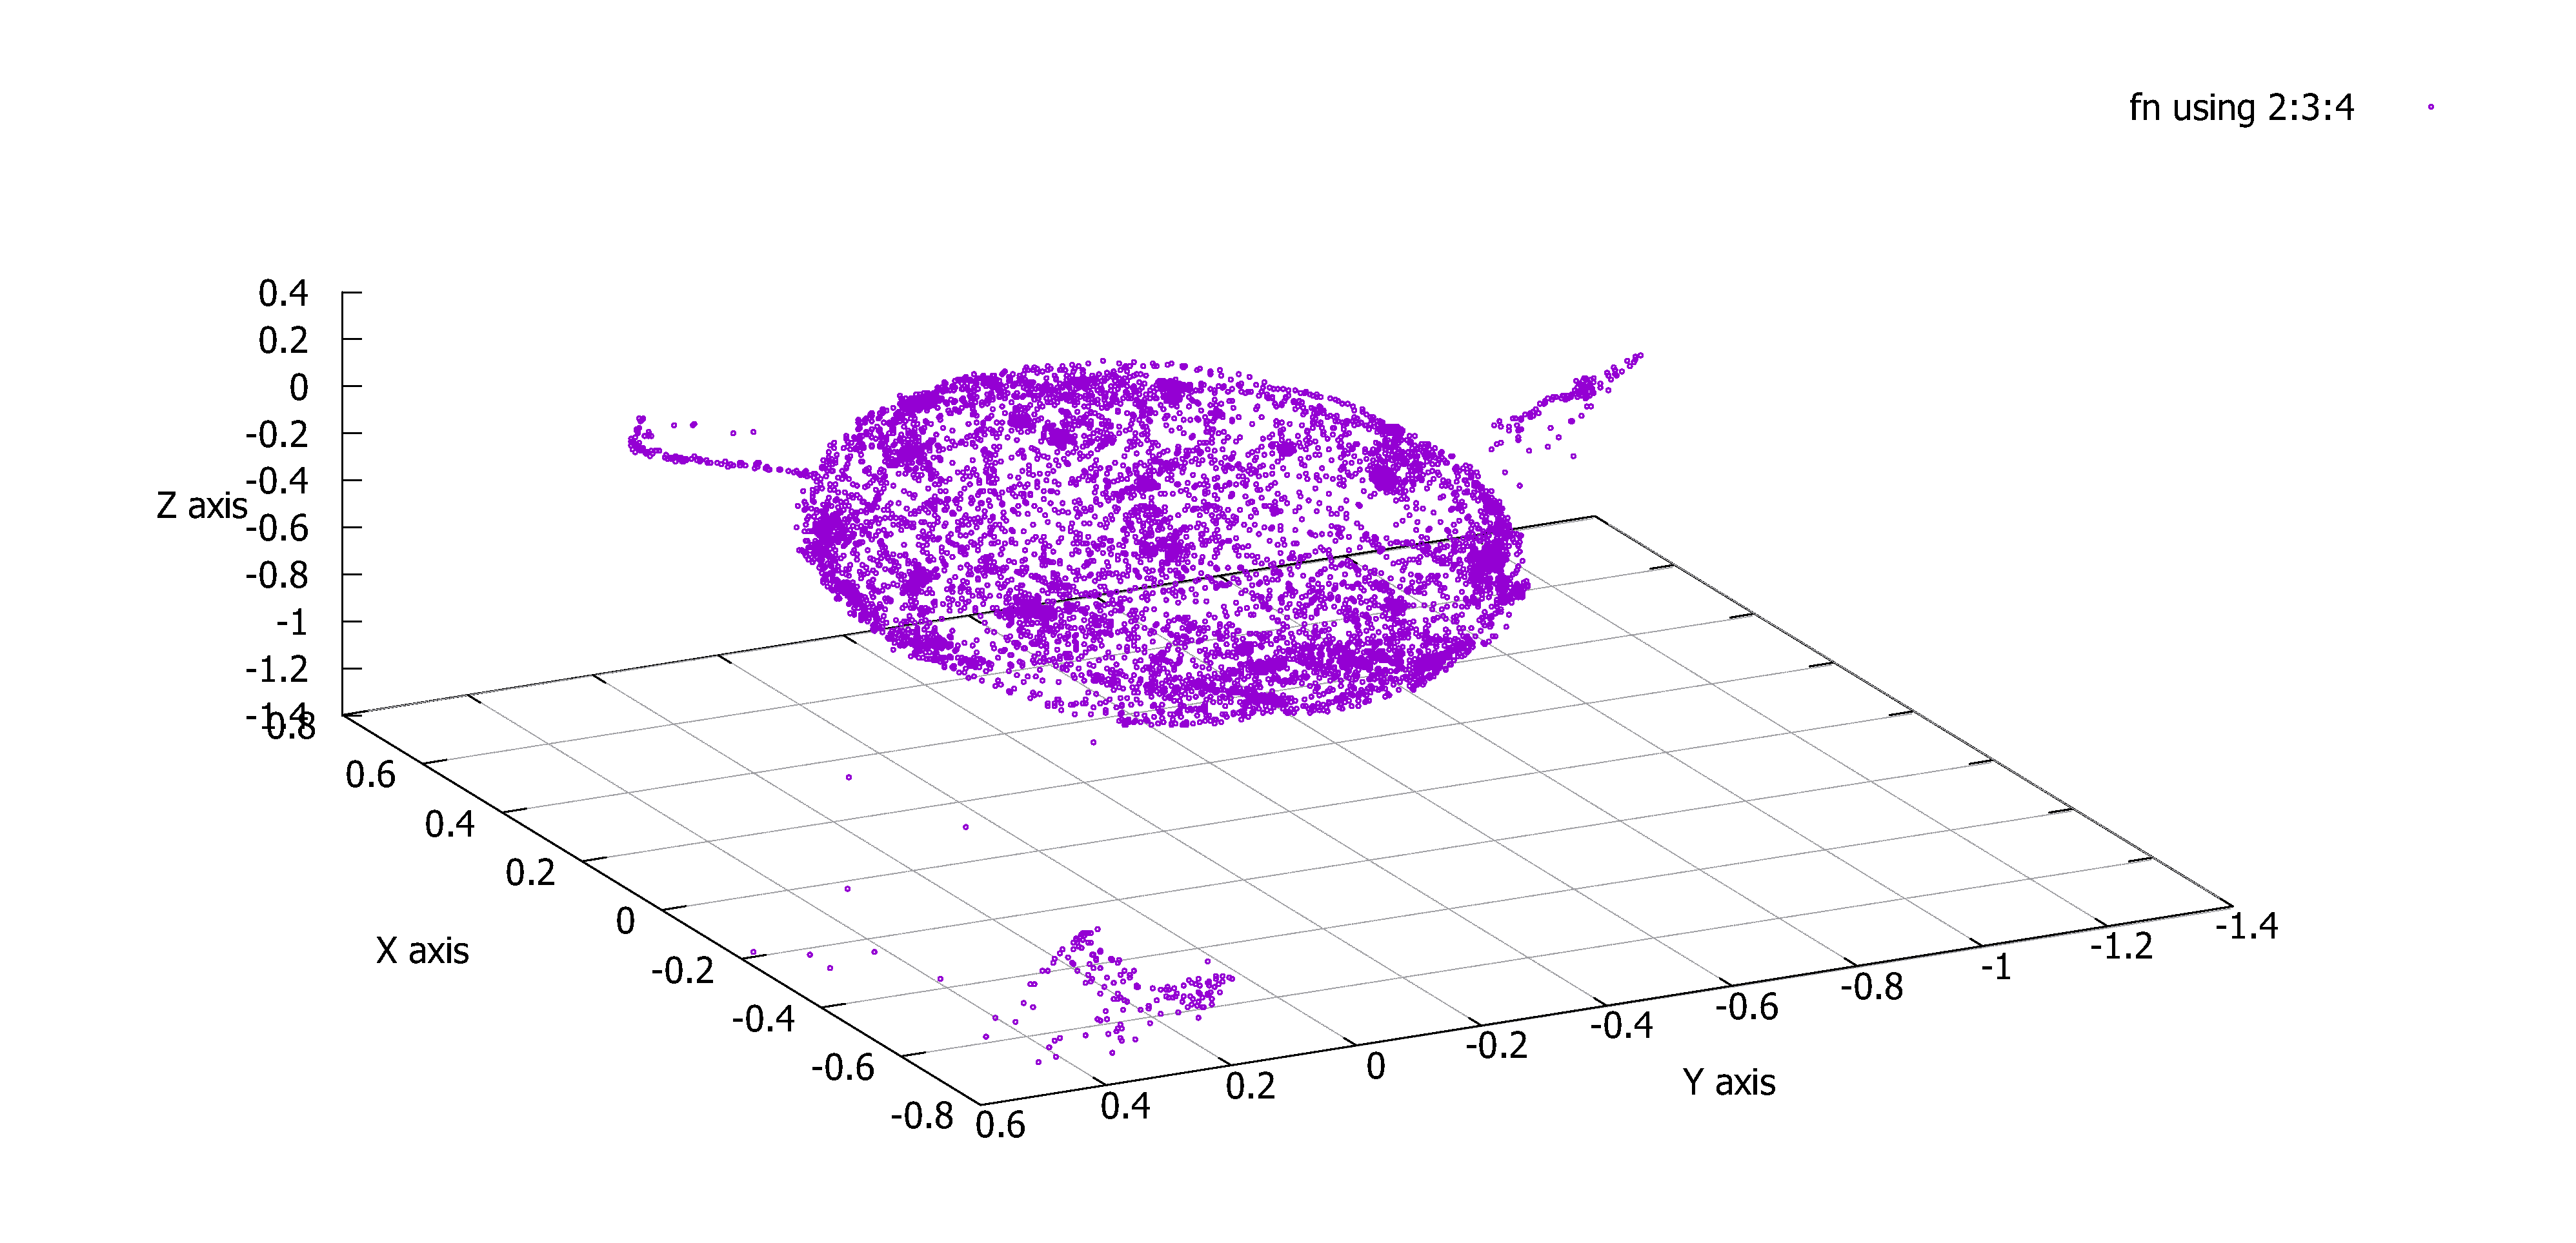
\includegraphics[width=.8\linewidth]{images/04_results/raw_sphere_2025-04-11.pdf}
%  \caption{2025-04-11}
%\end{subfigure}%
%\begin{subfigure}{.33\textwidth}
%  \centering
%  \includegraphics[width=.8\linewidth]{images/cali_mag_sphere_11apr.png}
%  \caption{2025-04-}
%\end{subfigure}
%\begin{subfigure}{.33\textwidth}
%  \centering
%  \includegraphics[width=.8\linewidth]{images/cali_mag_sphere_11apr.png}
%  \caption{2025-04-}
%\end{subfigure}
%\caption{Components of the magnetometer of the calibration measurements plotted in 3D-Space to form distorted spheres.}
%\label{fig:res:unfiltered_cali}
%\end{figure}


\section{Attitude \label{sec:res:attitude}}
In this section we evaluate the measurements of the accelerometer to determine roll and pitch angle of the gondola.

\section{Heading \label{sec:res:heading}}
This section will present the evaluation of the magnetometer as a means of determining the gondolas direction. The attitude of the gondola has to be taken into account beacuse...